\begin{frame}{Evaluations-Setup}

\end{frame}

\begin{frame}{Evaluation-Probleme}
\begin{description}
\item[\textbf{Soft N-Queens}] is a toy SCSP that adds three artificial soft constraints with a preference relation over them to a classical $N$-queens problem~(such as, e.g., having a queen in the center of the grid), not to be mistaken with the $M$-queens optimization problem.
\item[\textbf{Photo Placement}] asks to put in place people close to their friends -- in its original version it was already designed to handle preferences but we (morally questionably) allowed for some friends to be \emph{more important} to stand close to than others.
\item[\textbf{Talent Scheduling}] aims at scheduling movie scenes to be shot including various actors cost-effectively. We augmented the conventional problem with preferences to avoid being simultaneously on set with a rival actor and early/late times for specific scenes.
\item[\textbf{On-call Rostering}] requires to assign staff members to days in a rostering period, respecting work constraints and unavailabilities. The original formulation already contained preferences for not being on-call for more than two days in a row or not being on-call for a weekend and a consecutive day. We modeled these existing preferences in MiniBrass and added additional ones regarding preferred coworkers.
\item[\textbf{Multi-Skilled Project Scheduling}] (MSPSP) is a variant of resource-constrained project scheduling and asks to assign a set of tasks to workers such that the required set of skills for a task is provided by its assigned worker. To add soft constraints, we again allowed  workers to state with whom they would like to work and which tasks they would like to work on or which ones they would rather avoid.
\end{description}

\end{frame}

\begin{frame}{Solver-Vergleich auf Weighted CSP}
\begin{parchment}[Evaluationsfrage]
How fast and effectively (in terms of finding optima) can WCSP instances be solved by encoding them as COPs versus using a dedicated solver?
\end{parchment}
\end{frame}

\begin{frame}{Solver-Vergleich auf Weighted CSP I}
\vspace*{2ex}
\begin{table}
\centering
{
\scriptsize
\label{tab:resultsSolverComparison}

\begin{tabular*}{\textwidth}{@{\extracolsep{\fill} }ld{1.5}cd{1.5}d{1.1}d{1.1}}
\toprule
\multicolumn{1}{c}{Solver} & \multicolumn{1}{c}{Time (secs)} 
          & \multicolumn{1}{c}{\# Wins}
          & \multicolumn{1}{c}{Objective} 
          & \multicolumn{1}{c}{\% Solved} & \multicolumn{1}{c}{\% Optimal} \\
\midrule
\multicolumn{2}{l}{MSPSP (8 instances)  }   \\
\midrule
   Gecode & 0.32 \quad (1.00)& 8 & 2.50 \quad (0.00) & 100.00 & 100.00 \\
   G12 & 0.32 \quad (1.01)& 0 & 2.50 \quad (0.00) & 100.00 & 100.00 \\
   OR-Tools & 0.33 \quad (1.05)& 0 & 2.50 \quad (0.00) & 100.00 & 100.00 \\
   JaCoP & 0.52 \quad (1.73)& 0 & 2.50 \quad (0.00) & 100.00 & 100.00 \\
   Choco & 0.70 \quad (2.46)& 0 & 2.50 \quad (0.00) & 100.00 & 100.00 \\
   Toulbar2 & 312.56 \quad (1052.07)& 0 & 29.13 \quad (26.63) & 0.00 & 0.00 \\
\midrule
\multicolumn{2}{l}{On-Call Rostering (7 instances)  }   \\
\midrule
   Toulbar2 & 40.73 \quad (1.44)& 3 & 1.57 \quad (0.00) & 100.00 & 100.00 \\
   OR-Tools & 275.23 \quad (5.55)& 2 & 3.71 \quad (2.14) & 100.00 & 57.14 \\
   Gecode & 275.23 \quad (5.54)& 1 & 4.57 \quad (3.00) & 100.00 & 57.14 \\
   G12 & 276.36 \quad (5.63)& 1 & 5.57 \quad (4.00) & 100.00 & 57.14 \\
   JaCoP & 276.63 \quad (5.86)& 0 & 5.14 \quad (3.57) & 100.00 & 57.14 \\
   Choco & 276.72 \quad (6.26)& 0 & 5.14 \quad (3.57) & 100.00 & 57.14 \\
\midrule
\multicolumn{2}{l}{Photo Placement (3 instances)  }   \\
\midrule
   Toulbar2 & 0.80 \quad (1.11)& 0 & 13.33 \quad (0.00) & 100.00 & 100.00 \\
   Choco & 0.83 \quad (1.21)& 2 & 25.00 \quad (11.67) & 100.00 & 100.00 \\
   OR-Tools & 1.49 \quad (1.71)& 1 & 13.33 \quad (0.00) & 100.00 & 100.00 \\
   JaCoP & 3.18 \quad (3.61)& 0 & 13.33 \quad (0.00) & 100.00 & 100.00 \\
   Gecode & 22.24 \quad (21.62)& 0 & 13.33 \quad (0.00) & 100.00 & 100.00 \\
   G12 & 27.40 \quad (29.62)& 0 & 13.33 \quad (0.00) & 100.00 & 100.00 \\
\bottomrule
\end{tabular*}

}
\end{table}

\end{frame}

\begin{frame}{Solver-Vergleich auf Weighted CSP II}
\begin{table}
\centering
{
\scriptsize
\label{tab:resultsSolverComparison}

\begin{tabular*}{\textwidth}{@{\extracolsep{\fill} }ld{1.5}cd{1.5}d{1.1}d{1.1}}
\toprule
\multicolumn{1}{c}{Solver} & \multicolumn{1}{c}{Time (secs)} 
          & \multicolumn{1}{c}{\# Wins}
          & \multicolumn{1}{c}{Objective} 
          & \multicolumn{1}{c}{\% Solved} & \multicolumn{1}{c}{\% Optimal} \\
\midrule
\multicolumn{2}{l}{Soft N-Queens (3 instances)  }   \\
\midrule
   OR-Tools & 0.03 \quad (1.00)& 3 & 0.33 \quad (0.00) & 100.00 & 100.00 \\
   Toulbar2 & 0.30 \quad (10.43)& 0 & 0.33 \quad (0.00) & 100.00 & 100.00 \\
   Choco & 0.35 \quad (12.54)& 0 & 0.33 \quad (0.00) & 100.00 & 100.00 \\
   JaCoP & 57.22 \quad (1707.98)& 0 & 0.33 \quad (0.00) & 100.00 & 100.00 \\
   Gecode & 210.02 \quad (6266.00)& 0 & 1.67 \quad (1.33) & 100.00 & 66.67 \\
   G12 & 210.02 \quad (6266.14)& 0 & 1.67 \quad (1.33) & 100.00 & 66.67 \\
\midrule
\multicolumn{2}{l}{Talent Scheduling (7 instances)  }   \\
\midrule
   OR-Tools & 113.29 \quad (1.01)& 3 & 12.29 \quad (0.00) & 100.00 & 85.71 \\
   JaCoP & 117.71 \quad (1.84)& 0 & 12.29 \quad (0.00) & 100.00 & 85.71 \\
   Choco & 129.12 \quad (3.27)& 1 & 12.29 \quad (0.00) & 100.00 & 85.71 \\
   Toulbar2 & 158.27 \quad (60.70)& 0 & 28.43 \quad (16.14) & 28.57 & 28.57 \\
   Gecode & 183.29 \quad (4.70)& 3 & 12.29 \quad (0.00) & 100.00 & 85.71 \\
   G12 & 194.91 \quad (2.87)& 0 & 12.29 \quad (0.00) & 100.00 & 85.71 \\
\bottomrule
\end{tabular*}

}
\end{table}
\end{frame}

\begin{frame}{Vergleich Weighted vs Constraint Preferences}
\begin{parchment}[Evaluationsfrage]
Is optimizing according to the Smyth-ordering much more expensive than solving a weighted counterpart obtained by a morphism?
\end{parchment}
\end{frame}

\begin{frame}{Vergleich Weighted vs Constraint Preferences}
\vspace*{4ex}

\begin{table}
\centering
{
\scriptsize
\begin{tabular*}{\textwidth}{@{\extracolsep{\fill} }ld{1.1}d{1.1}d{1.1}d{1.1}d{1.1}}
\toprule
\multicolumn{1}{c}{Solver} & \multicolumn{1}{c}{Time Smyth} 
          & \multicolumn{1}{c}{Time Weighted} 
          & \multicolumn{1}{c}{Time Toulbar2}
          & \multicolumn{1}{c}{Obj. Weights} & \multicolumn{1}{c}{Obj. Smyth}   \\
\midrule
\multicolumn{2}{l}{MSPSP (6 instances)  }   \\
\midrule
   Gecode & 12.74 & \textbf{0}.\textbf{34} & - & 2.67 & 5.50 \\
   Native Gecode & 7.82 & \textbf{0}.\textbf{26} & - & 2.80 & 5.80 \\
   JaCoP & 4.18 & \textbf{0}.\textbf{45} & - & 2.00 & 6.00 \\
\midrule
\multicolumn{2}{l}{On-Call Rostering (5 instances)  }   \\
\midrule
   Gecode & 220.46 & \textbf{133}.\textbf{32} & 14.52 & 3.20 & 7.20 \\
   Native Gecode & 192.50 & \textbf{133}.\textbf{32} & 14.52 & 3.20 & 25.20 \\
   JaCoP & 194.06 & \textbf{135}.\textbf{28} & 14.52 & 3.20 & 26.80 \\
\midrule
\multicolumn{2}{l}{Photo Placement (3 instances)  }   \\
\midrule
   Gecode & 6.69 & \textbf{1}.\textbf{03} & 0.68 & 13.00 & 13.00 \\
   Native Gecode & \textbf{9}.\textbf{96} & 22.22 & 0.80 & 13.33 & 13.33 \\
   JaCoP & 15.73 & \textbf{3}.\textbf{18} & 0.80 & 13.33 & 13.33 \\
\midrule
\multicolumn{2}{l}{Soft N-Queens (3 instances)  }   \\
\midrule
   Gecode & \textbf{3}.\textbf{45} & 210.02 & 0.30 & 1.67 & 2.00 \\
   Native Gecode & \textbf{3}.\textbf{49} & 210.02 & 0.30 & 1.67 & 1.33 \\
   JaCoP & \textbf{3}.\textbf{94} & 57.22 & 0.30 & 0.33 & 1.00 \\
\midrule
\multicolumn{2}{l}{Talent Scheduling (6 instances)  }   \\
\midrule
   Gecode & \textbf{7}.\textbf{78} & 158.94 & - & 12.50 & 14.25 \\
   Native Gecode & \textbf{13}.\textbf{50} & 141.09 & - & 12.33 & 14.67 \\
   JaCoP & \textbf{15}.\textbf{63} & 120.42 & - & 12.33 & 14.17 \\
\bottomrule
\end{tabular*}

}
\end{table}
\end{frame}

\begin{frame}
\begin{table}
\centering
{
\scriptsize
\caption{Comparison of runtimes between searching for all optima instead of a strict domination improvement. 
We only considered \emph{solved} instances in this evaluation. Bold-face highlighting indicates the faster search type. Values are averaged over instances and solvers. }
\label{tab:compDomNonDom}


\begin{tabular*}{\textwidth}{@{\extracolsep{\fill} }ld{1.1}d{1.1}d{1.1}d{1.1}}
\toprule
\multicolumn{1}{c}{Problem} & \multicolumn{1}{c}{Time Non-Dominated BaB} 
          & \multicolumn{1}{c}{Time Strict BaB} 
          & \multicolumn{1}{c}{Absolute Overhead}
          & \multicolumn{1}{c}{Relative Overhead}   \\
\midrule
   MSPSP & \textbf{7}.\textbf{31} & 8.89 & -1.58 & 1.50 \\
   On-Call Rostering & 329.44 & \textbf{199}.\textbf{21} & 130.23 & 1.82 \\
   Photo Placement & 55.09 & \textbf{7}.\textbf{51} & 47.58 & 9.72 \\
   Soft N-Queens & \textbf{2}.\textbf{24} & 3.65 & -1.41 & 1.91 \\
   Talent Scheduling & 33.44 & \textbf{12}.\textbf{24} & 21.21 & 2.30 \\
\midrule
\emph{Overall} & 102.00 & \textbf{57}.\textbf{20} & 44.80 & 2.97 \\
\bottomrule
\end{tabular*}
}
\end{table}

\end{frame}

\begin{frame}{Vergleich MIF vs. Standard}
\begin{parchment}[Evaluationsfrage]
Can a generic heuristic (MIF) for soft constraint problems speed up the search for optima?
\end{parchment}
\end{frame}

\begin{frame}{Vergleich MIF vs. Standard I}
\begin{table}
\centering
{
\scriptsize

\label{tab:compDiffsMif}


\subcaption*{Grouped by solvers.}
\begin{tabular*}{\textwidth}{@{\extracolsep{\fill} }ld{1.1}d{1.1}d{1.1}d{1.1}d{1.1}d{1.1}d{1.1}}
\toprule
 &  \multicolumn{1}{c}{Choco} & \multicolumn{1}{c}{G12} & \multicolumn{1}{c}{Gecode} & \multicolumn{1}{c}{JaCoP} & \multicolumn{1}{c}{Toulbar2} & \multicolumn{1}{c}{OR-Tools} \\
\midrule
Instances &  28 & 28 & 28 & 28 & 28 & 28 \\
Runtime difference &  -73.14 & -17.57 & -18.42 & 16.15 & 36.63 & 19.05 \\
Ratio MIF wins &  0.64 & 0.32 & 0.29 & 0.46 & 0.57 & 0.32 \\
\bottomrule
\end{tabular*}

\bigskip
\subcaption*{Grouped by problems.}

\begin{tabular*}{\textwidth}{@{\extracolsep{\fill} }ld{1.1}d{1.1}d{1.1}d{1.1}d{1.1}d{1.1}}
\toprule
 &  \multicolumn{1}{c}{MSPSP} & \multicolumn{1}{c}{On-Call Rostering} & \multicolumn{1}{c}{Photo Placement} & \multicolumn{1}{c}{Soft N-Queens} & \multicolumn{1}{c}{Talent Scheduling} \\
\midrule
Instances &  48 & 42 & 18 & 18 & 42 \\
Runtime difference &  -0.80 & -31.04 & 141.17 & -79.51 & -19.34 \\
Ratio MIF wins &  0.42 & 0.55 & 0.06 & 0.56 & 0.45 \\
\bottomrule
\end{tabular*}
}
\end{table}
\end{frame}

\begin{frame}{Vergleich MIF vs. Standard II}
\begin{figure}
	\centering
	\begin{subfigure}[b]{.48\textwidth}
		\centering
		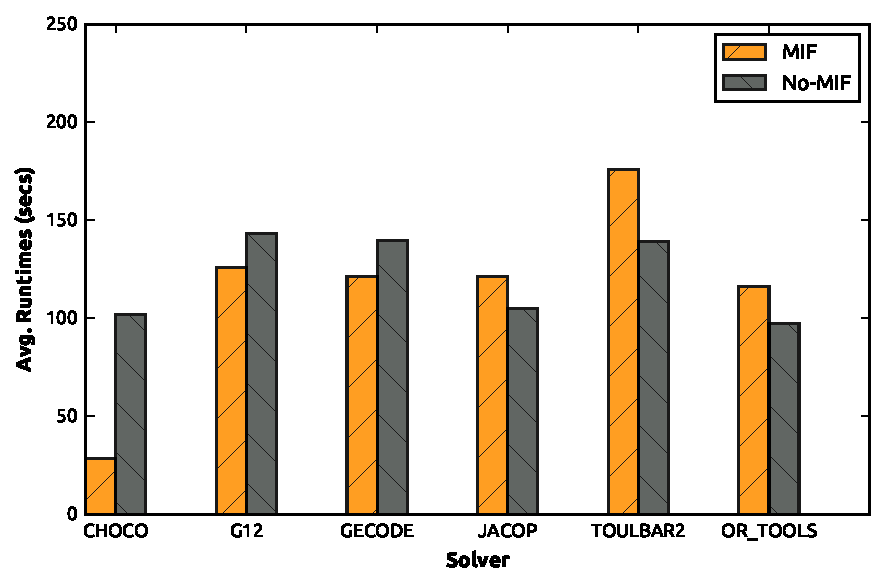
\includegraphics[width=\textwidth]{img/runtime-mif-solver.pdf} %TODO: check: how were the 8 points sampled? Not uniformly...
         \caption{Runtimes grouped by solver for MIF on/off.}
		\label{fig:runtimesMIFSolvers}
	\end{subfigure}%
	~ \quad%add desired spacing between images, e. g. ~, \quad, \qquad, \hfill etc.
	%(or a blank line to force the subfigure onto a new line)
	\begin{subfigure}[b]{.48\textwidth}
		\centering
		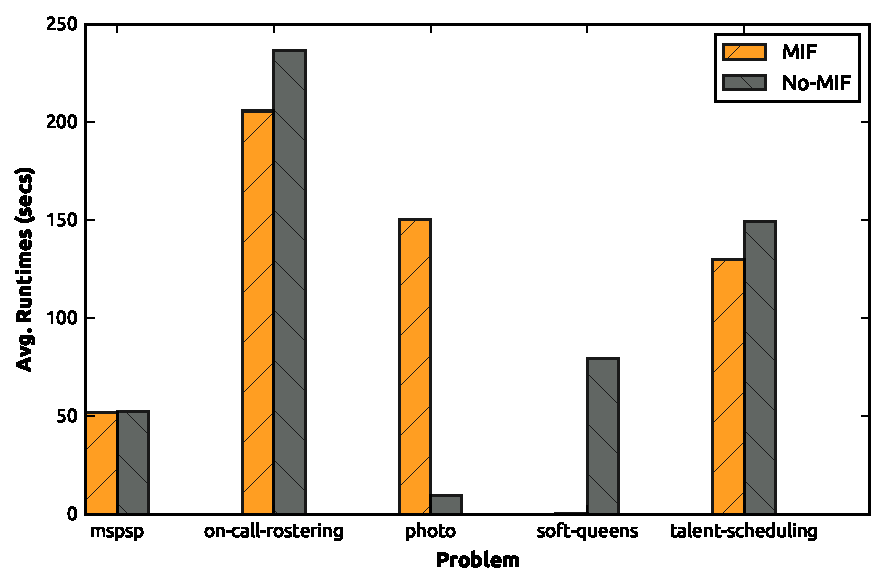
\includegraphics[width=\textwidth]{img/runtime-mif-problem.pdf}
		\caption{Runtimes grouped by problem for MIF on/off.}
		\label{fig:runtimesMIFProblems}
	\end{subfigure}

	\label{fig:runtimesMIF}
\end{figure}
\end{frame}